\section{Оптический отклик полупроводниковой метаповерхности на основе германия.}

\subsection{Постановка задачи. Параметры образца.}
В полупроводниковых наноструктурах с субволновым периодом решетки ожидаться резонанс в следствии многократного рассеяния  волны накачки \cite{mftiOpt}. В данной структуре (рис. \ref{base1}) ожидался резонанс в конце ИК диопазона.

\begin{figure}[h]
	\centering
    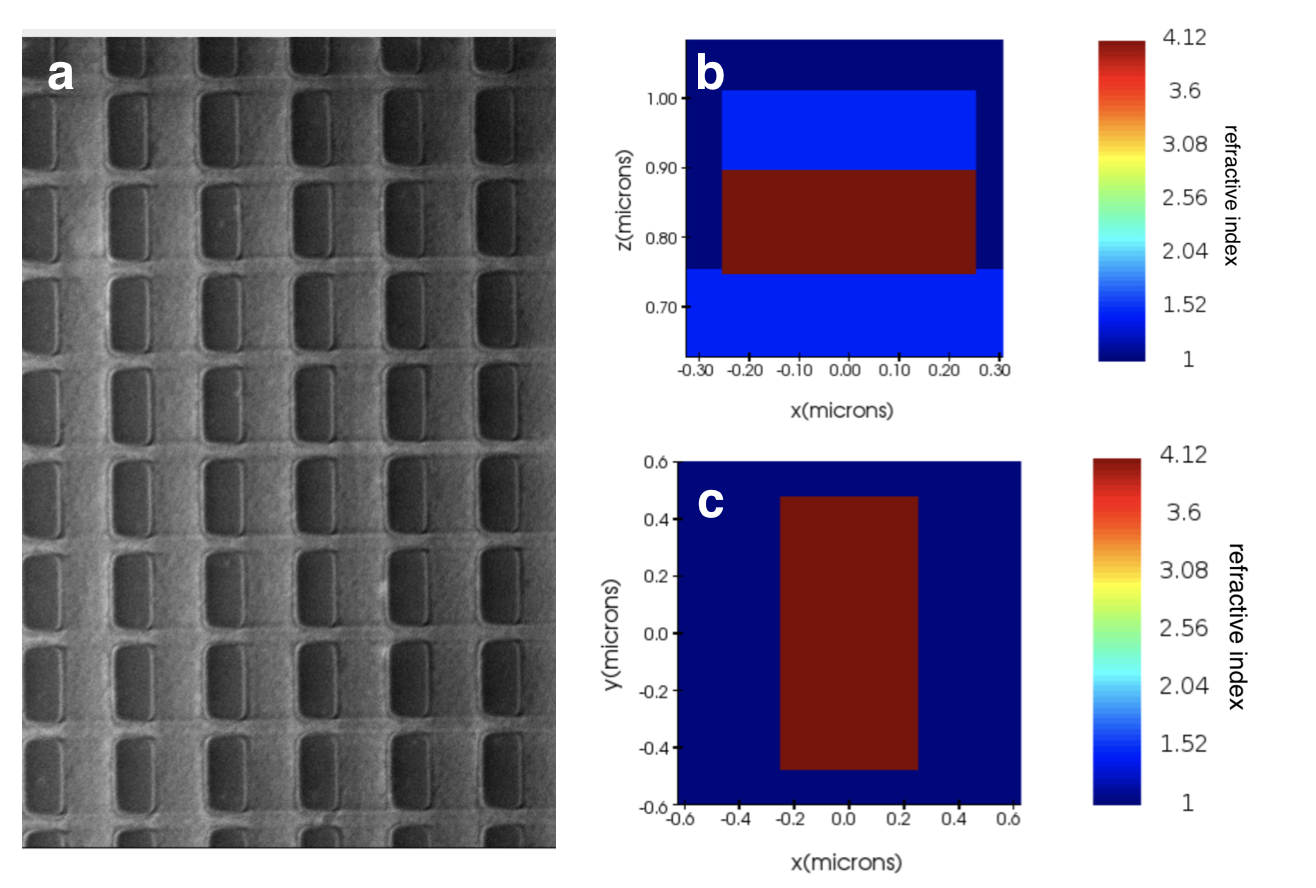
\includegraphics[width=0.8\linewidth]{images/base1.png}
	\caption{\textbf{(a)}На рисунке изображен снимок метаповерхности. В качестве подложки используется $CaF_2$. На подложке с шагом горизонтальным шагом 0,75мкм и вертикальным шагом 0,25мкм разположенны кирпичике германия(Ge) толщиной 0,15мкм. На верху каждого кирпичека германия расположен слой стекал ($SiO_2$) толщиной $\sim 0,1$мкм. \textbf{(b), (c)} - виды модели с боку и с верху соответственно. Цветная шкала справа показывает показатель преломления различных структур)}
	\label{base1}
\end{figure}

\subsection{Исследование линейного отклика метаповерхности на основе германия}
\hspace{2mm}
Периодическая структура освещаться плоской волной накачки. Монитор 1(рис 2а) расположен внутри кирпичика германия и измеряет пропускание структуры, а монитора 2(рис.  2а) расположен выше источника электромагнитных волн и измеряет отражение структуры. Резонанс (рис. 2b) можно наблюдать как на спектре пропускание(рис 2с) так и на отражения структуры (рис 2d) .  Из графиков видно, что резонанс достигаться на длине волны  $\lambda_{RES} \approx 2$мкм
%тут еще картинка а - скрин из проги, б - е-резонанс, с,d - пропускание отражение f - 2Dкартина разонанса
\hspace{2mm}
 Вероятнее всего наблюдаемый резонанс возникает из-за геометрических особенностей метаповерхности. В результате многократного отражения волны накачки генерируется квазиволновая мода, которую мы и наблюдаем в резонансе 



